\documentclass[serif]{beamer}
\usepackage[utf8]{inputenc}
\usepackage[T1]{fontenc}
\usepackage[french]{babel}

\usetheme[sectionpage=progressbar]{metropolis}

%============================================================

\usepackage{minted}
\usepackage{graphicx}
\usepackage{xspace}
\usepackage{caption}
\usepackage{textgreek}	% textmu

%============================================================

\usepackage{tikz}
\usetikzlibrary{automata,positioning}

%============================================================

\usepackage{listings}

\makeatletter
\newenvironment{btHighlight}[1][]
{\begingroup\tikzset{bt@Highlight@par/.style={#1}}\begin{lrbox}{\@tempboxa}}
{\end{lrbox}\bt@HL@box[bt@Highlight@par]{\@tempboxa}\endgroup}

\newcommand\btHL[1][]{%
  \begin{btHighlight}[#1]\bgroup\aftergroup\bt@HL@endenv%
}
\def\bt@HL@endenv{%
  \end{btHighlight}%   
  \egroup
}
\newcommand{\bt@HL@box}[2][]{%
  \tikz[#1]{%
    \pgfpathrectangle{\pgfpoint{1pt}{0pt}}{\pgfpoint{\wd #2}{\ht #2}}%
    \pgfusepath{use as bounding box}%
    \node[anchor=base west, fill=orange!30,outer sep=0pt,inner xsep=1pt, inner ysep=0pt, rounded corners=3pt, minimum height=\ht\strutbox+1pt,#1]{\raisebox{1pt}{\strut}\strut\usebox{#2}};
  }%
}
\makeatother

\lstset{
	basicstyle=\ttfamily,
	columns=fullflexible,
	keepspaces=true,
	moredelim=**[is][\btHL]{`}{`},
	extendedchars=true,
	literate={µ}{{\textmu}}1
}

%============================================================

\usepackage{amsmath}	% align*
\usepackage{amssymb}	% mathbb
\usepackage{mathrsfs}	% mathscr
\usepackage{scalerel}	% scalerel
\usepackage{mathtools}	% mathclap

%============================================================

\usepackage{mathpartir}
\def\RightTirNameStyle{\textnormal}

%============================================================

\newcommand{\dowsindex}{\texttt{dowsindex}\xspace}
\newcommand{\exemple}{\textit{Exemple}\xspace}
\newcommand{\exemples}{\textit{Exemples}\xspace}
\newcommand{\theoreme}{\textit{Théorème}\xspace}

\newcommand{\interval}[2]{[\![#1\,;#2]\!]}
\newcommand{\mset}[1]{\{\![#1]\!\}}

\newcommand{\qeq}{\stackrel {\scriptscriptstyle ?} =}

\newcommand{\ssi}{\textit{ssi}\xspace}
\newcommand{\unit}{\bold{unit}}
\newcommand{\norm}{\mathrm{norm}}

\newcommand{\V}{\mathscr{V}}
\newcommand{\F}{\mathscr{F}}
\newcommand{\E}{\mathscr{E}}
\newcommand{\G}{\mathscr{G}}
\newcommand{\T}{\mathrm{T}}
\newcommand{\N}{\mathrm{N}}

\newcommand{\mathhyphen}{{\hbox{-}}}

\DeclareMathOperator*{\msetN_bigplus}{\scalerel*{+}{\sum}^\#_\N}
\DeclareMathOperator*{\msetG_bigplus}{\scalerel*{+}{\sum}^\#_\G}

%============================================================

\title{Recherche de fonctions par \\ unification modulo isomorphismes de types}
\author{Clément ALLAIN \\ Stage de M1 encadré par Gabriel RADANNE et Laure GONNORD}
\date{\today}

%============================================================

\begin{document}

%============================================================

\begin{frame}
\titlepage
\end{frame}

%============================================================

\begin{frame}
\tableofcontents
\end{frame}

%============================================================
%============================================================

\section{Préambule}

%============================================================

\begin{frame}{Recherche de fonctions}
\begin{figure}[h]
 	\centering
 	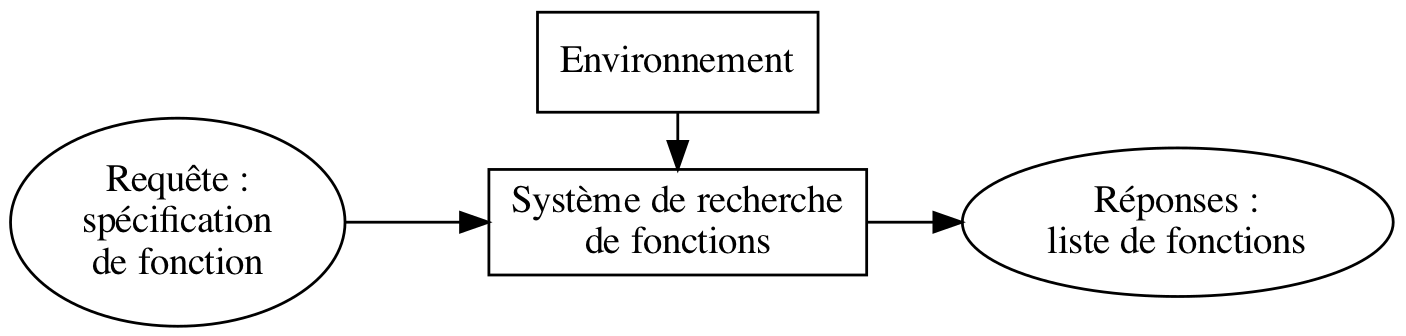
\includegraphics[scale=0.2]{graphs/recherche_fonction}
\end{figure}
\centering
Spécification de fonction ?
\end{frame}

%============================================================

\begin{frame}{Spécification de fonction}
\footnotesize
\begin{table}[h]
 	\centering
 	\begin{tabular}{|l|l|l|}
	 	\hline
	 		Langage &
			Nom &
			Type
		\\
		\hline
			LCF ML &
			\texttt{itlist} &
			$(\alpha \rightarrow \beta \rightarrow \beta) \rightarrow list (\alpha) \rightarrow \beta \rightarrow \beta$
		\\
			Caml Light &
			\texttt{list\_it} &
			$(\alpha \rightarrow \beta \rightarrow \beta) \rightarrow list (\alpha) \rightarrow \beta \rightarrow \beta$
		\\
			Haskell &
			\texttt{foldr} &
			$(\alpha \rightarrow \beta \rightarrow \alpha) \rightarrow \alpha \rightarrow list (\beta) \rightarrow \alpha$
		\\
			SML of New Jersey &
			\texttt{fold} &
			$(\alpha \times \beta \rightarrow \beta) \rightarrow list (\alpha) \rightarrow \beta \rightarrow \beta$
		\\
			Edinburgh SML &
			\texttt{fold\_right} &
			$(\alpha \times \beta \rightarrow \beta) \rightarrow \beta \rightarrow list (\alpha) \rightarrow \beta$
		\\
		\hline
	\end{tabular}
	\caption*{Variations sur \texttt{List.fold\_left} d'OCaml dans plusieurs dialectes de Core-ML \footnote{M. Rittri : \textit{Using types as search keys in function libraries} (1991).}.}
\end{table}
\end{frame}

%============================================================

\begin{frame}[fragile=singleslide]\frametitle{\dowsindex}
\begin{figure}[h]
 	\centering
 	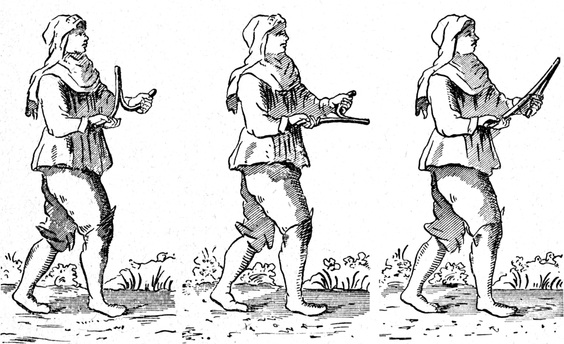
\includegraphics{images/sourcier}
\end{figure}
\footnotesize
\begin{verbatim}
	$ ./dowsindex search "'a list * 'a -> bool"
	...
	List.mem : 'a -> 'a list -> bool
	...
	$ ./dowsindex search "'a list -> ('a * 'b -> 'b) -> 'b -> 'b"
	...
	List.fold_left : ('a -> 'b -> 'a) -> 'a -> 'b list -> 'a
	List.fold_right : ('a -> 'b -> 'b) -> 'a list -> 'b -> 'b
	...
\end{verbatim}
\end{frame}

%============================================================
%============================================================

\section{Unification modulo isomorphismes de types}

%============================================================

\begin{frame}[fragile=singleslide]\frametitle{Intuition}
\small
\[ \mintinline{ocaml}{'a list * 'a -> bool}\ \ \sim\ \ \mintinline{ocaml}{'a -> 'a list -> bool} \]
\smallskip
\[ \mintinline{ocaml}{'a * 'b -> 'c}\ \ \sim\ \ \mintinline{ocaml}{'a -> 'b -> 'c} \]
\begin{minted}{ocaml}
# let curry f a b = f (a, b) ;;
val curry : ('a * 'b -> 'c) -> 'a -> 'b -> 'c = <fun>
# let uncurry f (a, b) = f a b ;;
val uncurry : ('a -> 'b -> 'c) -> 'a * 'b -> 'c = <fun>
\end{minted}
\bigskip
\[ \mintinline{ocaml}{'a -> 'b -> 'c} \ \ \sim\ \ \mintinline{ocaml}{'b -> 'a -> 'c} \]
\begin{minted}{ocaml}
# let flip f a b = f b a ;;
val flip : ('a -> 'b -> 'c) -> 'b -> 'a -> 'c = <fun>
\end{minted}
\end{frame}

%============================================================

\begin{frame}{Types}
\begin{mathpar}
    \inferrule* 
    	{ }
    	{\V \subseteq \T}
    \and
    \inferrule*
    	{ }
    	{\unit \in \T}
    \\
    \inferrule*
    	{\tau_1 \in \T \\ \tau_2 \in \T}
    	{\tau_1 \times \tau_2 \in \T}
    \and
   	\inferrule*
   		{\tau_1 \in \T \\ \tau_2 \in \T}
   		{\tau_1 \rightarrow \tau_2 \in \T}
   	\and
    \inferrule*
    	{f \in \F \\ \overline\tau \in \T^{|f|_\F}}
    	{f (\overline\tau) \in \T}
\end{mathpar}
\exemples :
\begin{itemize}
	\item $\unit \rightarrow int \times float$
	\item $int \rightarrow (int \rightarrow \alpha) \rightarrow array (\alpha)$
	\item $(\alpha \rightarrow \beta \rightarrow \alpha) \rightarrow \alpha \rightarrow list (\beta) \rightarrow \alpha$
\end{itemize}
\end{frame}

%============================================================

\begin{frame}{Isomorphismes de types dans $\Lambda^1$}
Deux types $\tau_1$ et $\tau_2$ sont \emph{isomorphes} dans $\Lambda^1$ \ssi le diagramme suivant commute :
\begin{figure}[h]
 	\centering
	\begin{tikzpicture}[shorten >=1pt,node distance=2cm,on grid,auto]
		\node[state] (ty1) {$\tau_1$} ;
		\node[state] (ty2) [right=of ty1] {$\tau_2$} ;
		\path[->]
			(ty1)
				edge [dotted, bend left] node {$f : \tau_1 \rightarrow \tau_2$} (ty2)
				edge [loop left] node {$\mathrm{id}_{\tau_1}$} ()
			(ty2)
				edge [dotted, bend left] node {$g : \tau_2 \rightarrow \tau_1$} (ty1)
				edge [loop right] node {$\mathrm{id}_{\tau_2}$} () ;
	\end{tikzpicture}
\end{figure}
\end{frame}

%============================================================

\begin{frame}{Théorie équationnelle $\E$}
\small
Système équationnel $\E$ :
\begin{align}
		\alpha \times \beta &\cong_\T
		\beta \times \alpha
		\label{prod_comm}
		\tag{$\times$-comm}
	\\
		\alpha \times (\beta \times \gamma) &\cong_\T
		(\alpha \times \beta) \times \gamma
		\label{prod_assoc}
		\tag{$\times$-assoc}
	\\
		\unit \times \alpha &\cong_\T
		\alpha
		\label{prod_unit}
		\tag{$\times$-$\unit$}
	\\
		(\alpha \times \beta) \rightarrow \gamma &\cong_\T
		\alpha \rightarrow (\beta \rightarrow \gamma)
		\label{curry}
		\tag{curry}
\end{align}
$\equiv_\T$ : plus petite congruence contenant toutes les instances des axiomes de $\E$.
\begin{itemize}
	\item $int \rightarrow float \rightarrow int \equiv_\T float \rightarrow int \rightarrow int$
	\item $int \rightarrow \unit \rightarrow \unit \equiv_\T int \rightarrow \unit$
	\item $int \rightarrow (int \times int) \rightarrow \unit \equiv_\T int \rightarrow int \rightarrow int \rightarrow \unit$
\end{itemize}
\end{frame}

%============================================================

\begin{frame}{Unifiabilité}
\small
Deux types $\tau_1$ et $\tau_2$ sont \emph{unifiables}, noté $\tau_1 \sim_\T \tau_2$, \ssi ils admettent un \emph{unificateur}, c'est-à-dire une substitution $\sigma$ telle que :
\[ \hat\sigma (\tau_1) \equiv_\T \hat\sigma (\tau_2) \]
\begin{itemize}
	\item $int \rightarrow float \rightarrow int \sim_\T float \rightarrow \alpha$ \\ avec $\{ \alpha \mapsto int \rightarrow int \}$
	\item $int \rightarrow \alpha \rightarrow \unit \sim_\T int \rightarrow \unit$ \\ avec $\{ \alpha \mapsto \unit \}$
	\item $int \rightarrow \alpha \rightarrow \unit \sim_\T int \rightarrow int \rightarrow int \rightarrow \unit$ \\ avec $\{ \alpha \mapsto int \times int \}$
\end{itemize}
\end{frame}

%============================================================
%============================================================

\section{Indexation}

%============================================================

\begin{frame}[fragile=singleslide]\frametitle{Recherche naïve}
\begin{verbatim}
$ ./dowsindex stats --no-index "int -> int -> int"
...
total time (s): 11.0211
total # unif.: 1638855
\end{verbatim}
\end{frame}

%============================================================

\begin{frame}[fragile=singleslide]\frametitle{Recherche avec mémoïsation}
\begin{verbatim}
$ ./dowsindex save
$ ./dowsindex stats "int -> int -> int"
...
total time (s): 0.595286
total # unif.: 31578
\end{verbatim}
\end{frame}

%============================================================

\begin{frame}[fragile=singleslide]\frametitle{Recherche avec mémorisation — requête plus difficile}
\begin{verbatim}
$ ./dowsindex stats "int -> int -> int -> int -> int"
...
total time (s): 58.2352
total # unif.: 31578
\end{verbatim}
\end{frame}

%============================================================

\begin{frame}[fragile=singleslide]\frametitle{Première métrique : nombre de variables uniques}
\scriptsize
\begin{itemize}
	\item $\mu^1 (\alpha \rightarrow \alpha) = 1$
	\item $\mu^1 (\alpha \rightarrow list (\beta) \rightarrow (\unit \rightarrow \beta) \rightarrow \alpha) = 2$
\end{itemize}
\begin{lstlisting}
$ ./dowsindex stats "int -> int -> int" --measure unique-vars
--------------------------------------------------------
measure    total time (ms)    avg. time (µs)    # unif.
--------------------------------------------------------
0          28.1541            1.48948            `18902`
1          108.248            15.2291            `7108`
2          373.408            `108.015`            3457
3          16.8808            11.8295            1427
4          7.12752            18.4174            387
...
--------------------------------------------------------
total time (s): 0.555204
total # unif.: 31578
\end{lstlisting}
\textit{Observation}. 0 variable : 60\% ; 1 variable : 20\%
\end{frame}

%============================================================

\begin{frame}[fragile=singleslide]\frametitle{Deuxième métrique : forme de la tête}
\scriptsize
\begin{itemize}
	\item $\mu^2 (\unit \rightarrow \alpha) = \bold{var}$
	\item $\mu^2 (int \rightarrow int \rightarrow list (\alpha)) = \bold{cons}_{list}$
\end{itemize}
\begin{lstlisting}
$ ./dowsindex stats "int -> int -> int" --measure head
------------------------------------------------------------
measure        total time (ms)    avg. time (µs)    # unif.
------------------------------------------------------------
variable       506.137            `311.086`            `1627`
constructor    62.705             2.45229            25570
tuple          11.2598            2.73429            4118
other          0.815153           3.09944            263
------------------------------------------------------------
total time (s): 0.580917
total # unif.: 31578
\end{lstlisting}
\textit{Observation}. $\bold{var}$ : 5\%
\end{frame}

%============================================================

\begin{frame}[fragile=singleslide]\frametitle{Troisième métrique : nombre de variables à la base}
\scriptsize
\begin{itemize}
	\item $\mu^3 (\alpha \times int) = 0$
	\item $\mu^3 ((\alpha \rightarrow \alpha) \rightarrow \alpha \rightarrow list (\alpha)) = 1$
\end{itemize}
\begin{lstlisting}
$ ./dowsindex stats "int -> int -> int" --measure spine-vars
--------------------------------------------------------
measure    total time (ms)    avg. time (µs)    # unif.
--------------------------------------------------------
0          70.9665            2.4932             `28464`
1          95.8333            44.6567            2146
2          397.937            486.476            818
3          5.00131            53.7775            93
...
--------------------------------------------------------
total time (s): 0.571445
total # unif.: 31578
\end{lstlisting}
\textit{Observation}. 0 variable : 90\%
\end{frame}

%============================================================

\begin{frame}{Conclusion métriques}
TODO
\end{frame}

%============================================================

\begin{frame}{Critère d'unifiabilité correct}
Critère d'unifiabilité correct sur $\mathscr{D}$ :
\begin{itemize}
	\item $encode : \T \rightarrow \mathscr{D}$
	\item $compat : \mathscr{D} \times \mathscr{D} \rightarrow \mathbb{B}$
	\item $compat (encode (\tau_1), encode (\tau_2)) = \bold{F} \implies \tau_1 \nsim_\T \tau_2$
\end{itemize}
\end{frame}

%============================================================

\begin{frame}{Premier critère}
Si deux types normalisés bien formés unifiables ne sont pas des variables, leurs têtes ont le même genre.
\\~\\
\exemples :
\begin{itemize}
	\item $\unit \rightarrow int \nsim_\T \unit \rightarrow float$
	\item $\unit \rightarrow int \nsim_\T \unit \rightarrow int \times int$
\end{itemize}
\end{frame}

%============================================================

\begin{frame}{Premier critère — implémentation}
\begin{figure}[h]
	\centering
	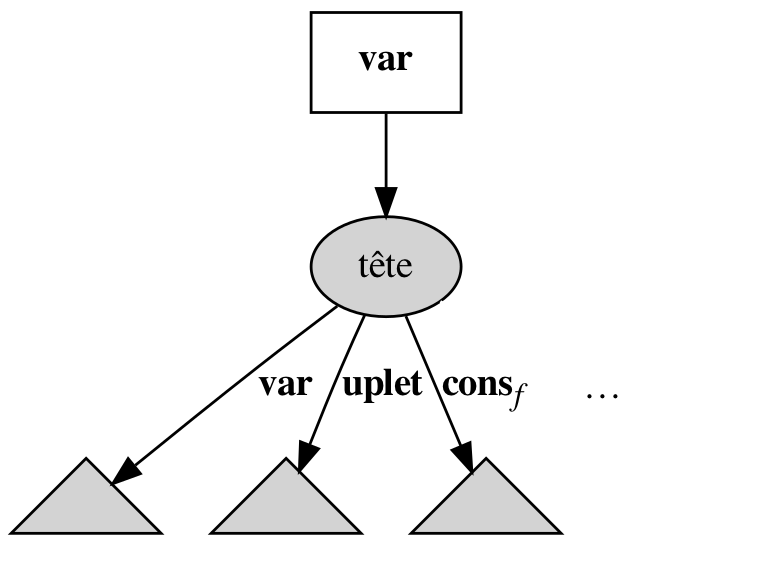
\includegraphics[scale=0.12]{graphs/crit1_1}
	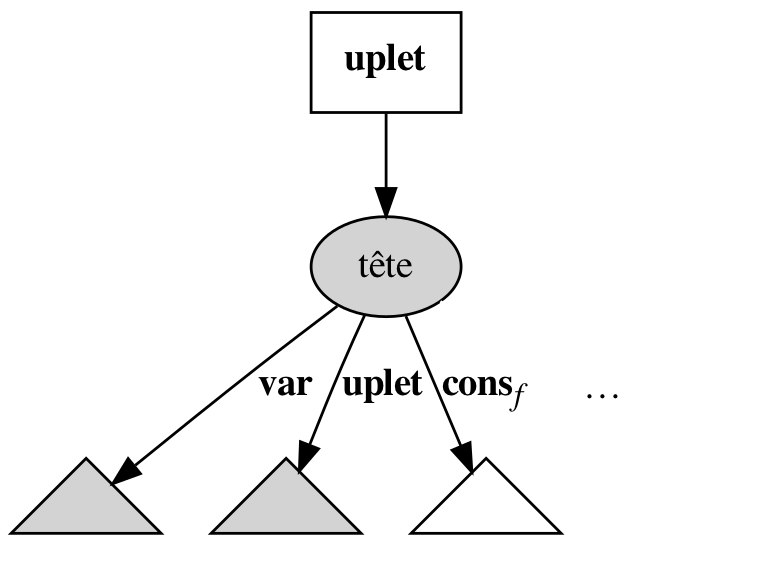
\includegraphics[scale=0.12]{graphs/crit1_2}
	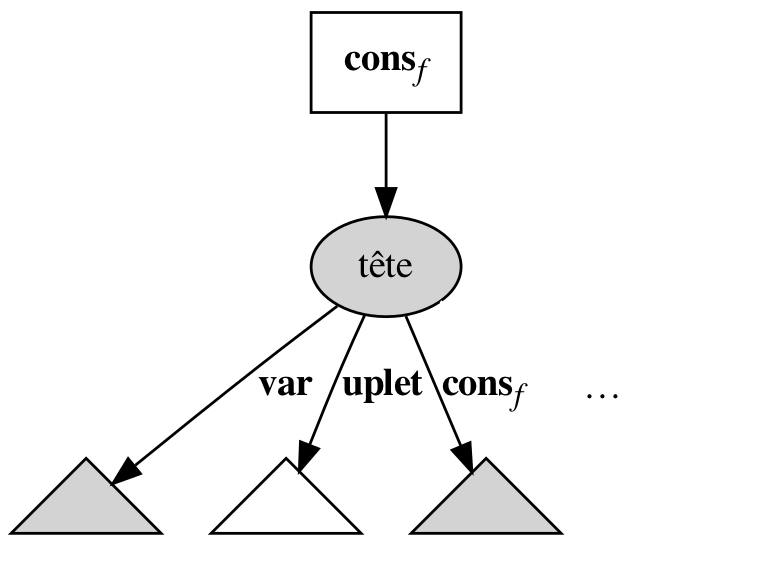
\includegraphics[scale=0.12]{graphs/crit1_3}
\end{figure}
\end{frame}

%============================================================

\begin{frame}[fragile=singleslide]\frametitle{Premier critère — apport}
\scriptsize
\begin{verbatim}
$ ./dowsindex save --index index.db --features head
$ ./dowsindex stats --index index.db --features head --with-features <type>
\end{verbatim}
\small
\begin{table}[h]
	\centering
	\begin{tabular}{|*{4}{c|}}
		\hline
			Type &
			\multicolumn{2}{c|}{Nombre d'unifications\dots} &
			Gain
		\\
		\cline{2-3}
      		&
			sans critère & avec critère &
		\\
		\hline
			$int \rightarrow int \rightarrow int$ &
			31578 & 2714 & 91.4\%
		\\
			$int \rightarrow int \rightarrow int \rightarrow int$ &
			31578 & 2714 & 91.4\%
		\\
			$int \rightarrow (int \rightarrow int) \rightarrow list (\alpha)$ &
			31578 & 2945 & 90.7\%
		\\
			$int \rightarrow float \rightarrow bool \rightarrow \bold{unit}$ &
			31578 & 5745 & 81.8\%
		\\
			$\alpha \rightarrow int \rightarrow \bold{unit}$ &
			31578 & 5745 & 81.8\%
		\\
			$int \rightarrow int \rightarrow \alpha$ &
			31578 & 31578 & 0\%
		\\
		\hline
	\end{tabular}
\end{table}
\end{frame}

%============================================================

\begin{frame}{Deuxième critère}
Si deux types normalisés bien formés $\tau_1$ et $\tau_2$ sont unifiables et $\tau_1$ n'a pas de variables à la base, la multiplicité de tout genre différent de $\bold{var}$ dans $\tau_1$ est supérieure à celle dans $\tau_2$.
\\~\\
\exemples :
\begin{itemize}
	\item
		$int \rightarrow int \rightarrow int \nsim_\T$ \\
		$int \rightarrow float$
	\item
		$int \rightarrow int \nsim_\T$ \\
		$int \rightarrow int \rightarrow \alpha \rightarrow \alpha$
	\item
		$int \rightarrow (\unit \rightarrow \unit) \rightarrow \unit \nsim_\T$ \\
		$int \rightarrow (int \rightarrow float) \rightarrow int \rightarrow \alpha$
\end{itemize}
\end{frame}

%============================================================

\begin{frame}{Deuxième critère — implémentation}
\begin{figure}[h]
	\centering
	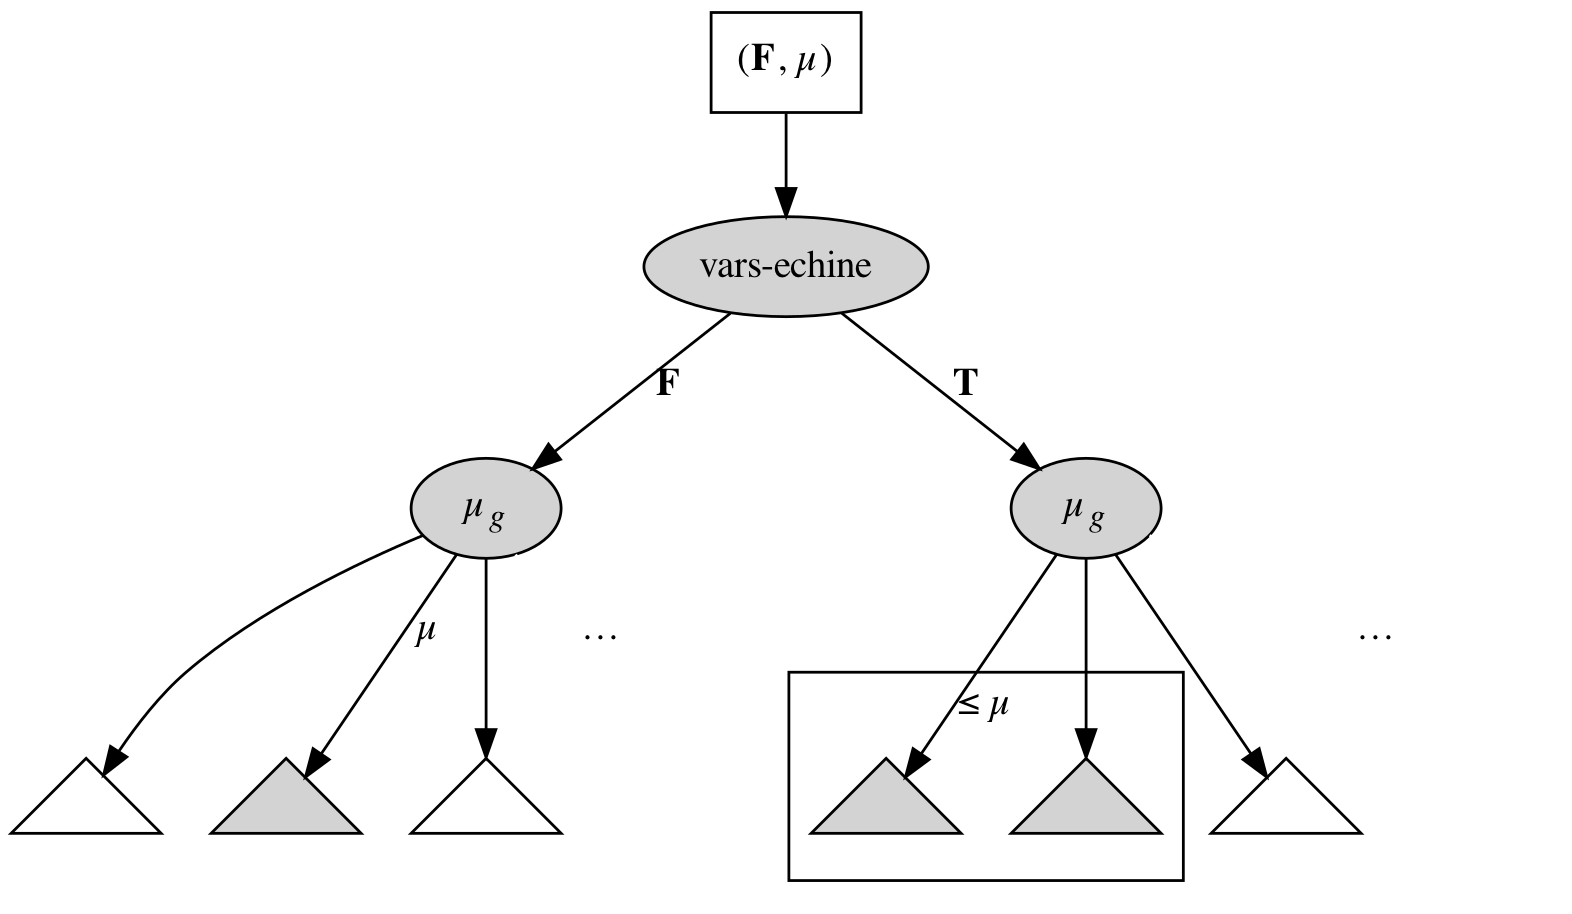
\includegraphics[scale=0.12]{graphs/crit2_1}
	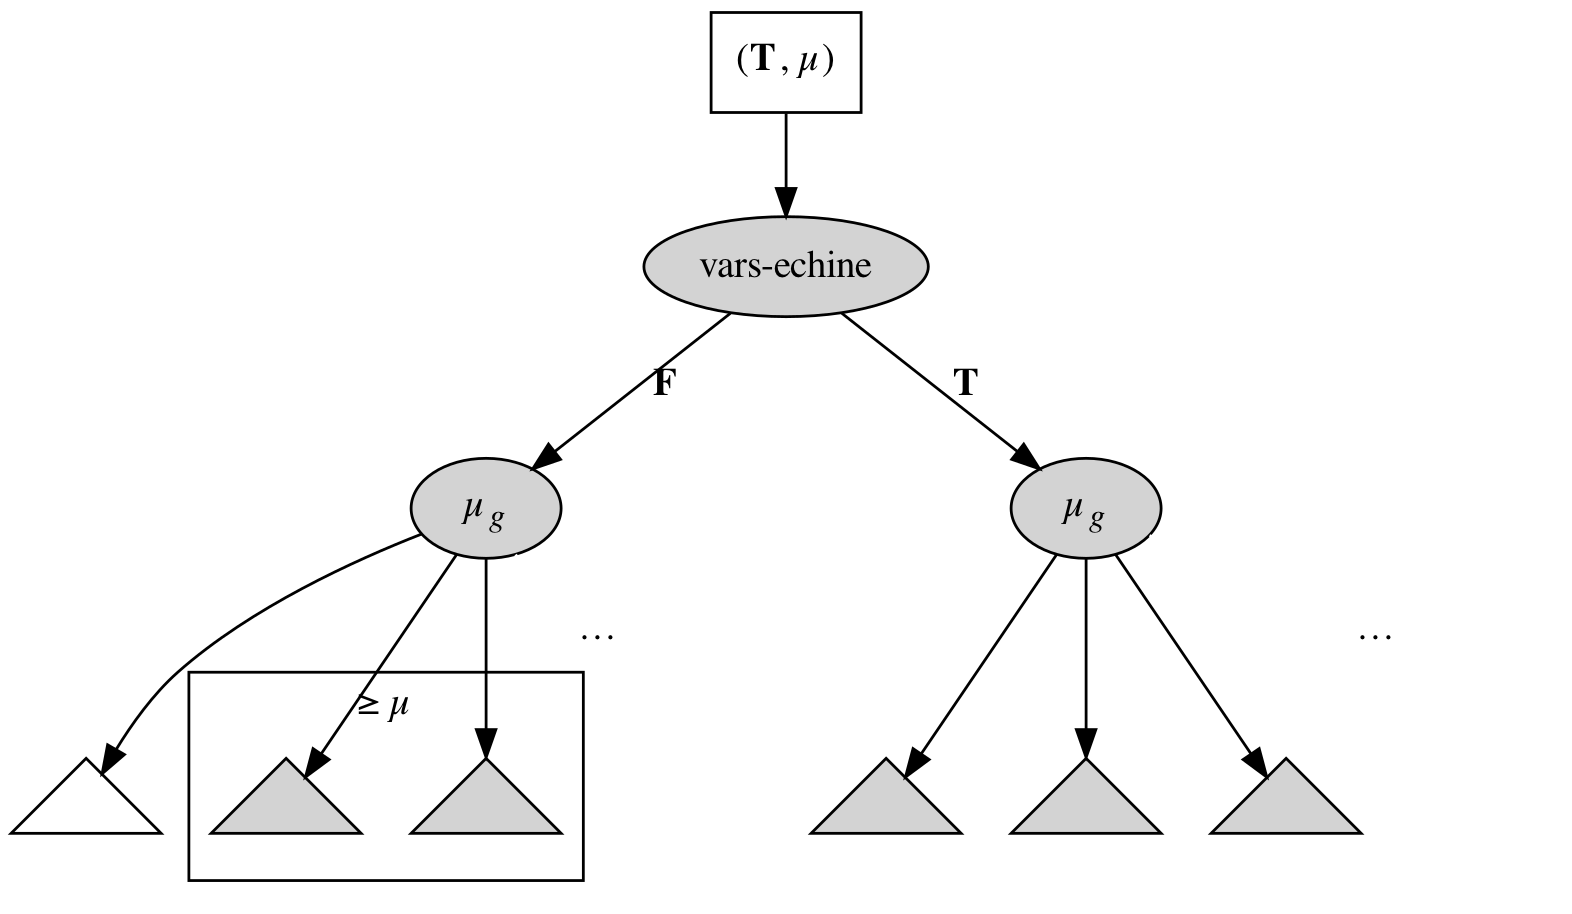
\includegraphics[scale=0.12]{graphs/crit2_2}
\end{figure}
\end{frame}

%============================================================

\begin{frame}[fragile=singleslide]\frametitle{Deuxième critère — apport}
\small
\begin{verbatim}
$ ./dowsindex stats --with-features <type>
\end{verbatim}
\begin{table}[h]
	\centering
	\begin{tabular}{|*{4}{c|}}
		\hline
			Type &
			\multicolumn{2}{c|}{Nombre d'unifications\dots} &
			Gain
		\\
		\cline{2-3}
			&
			sans critères & avec critères &
		\\
		\hline
			$int \rightarrow int \rightarrow int$ &
			31578 & 121 & 99.62\%
		\\
			$int \rightarrow int \rightarrow int \rightarrow int$ &
			31578 & 107 & 99.66\%
		\\
			$int \rightarrow (int \rightarrow int) \rightarrow list (\alpha)$ &
			31578 & 141 & 99.55\%
		\\
			$int \rightarrow float \rightarrow bool \rightarrow \bold{unit}$ &
			31578 & 126 & 99.6\%
		\\
			$\alpha \rightarrow int \rightarrow \bold{unit}$ &
			31578 & 2443 & 92.26\%
		\\
			$int \rightarrow int \rightarrow \alpha$ &
			31578 & 3677 & 88.36\%
		\\
		\hline
	\end{tabular}
\end{table}
\end{frame}

%============================================================

\begin{frame}{Conclusion critères}
TODO
\end{frame}

%============================================================

\begin{frame}[fragile=singleslide]\frametitle{\dowsindex}
\small
\begin{verbatim}
$ ./dowsindex search stdlib "'a list * 'a -> bool"
Parsing.is_current_lookahead : 'a -> bool
Obj.magic : 'a -> 'b
List.mem : 'a -> 'a list -> bool
List.memq : 'a -> 'a list -> bool
ListLabels.mem : 'a -> set:'a list -> bool
ListLabels.memq : 'a -> set:'a list -> bool
Compenv.print_version_string : unit -> 'a
Compenv.print_standard_library : unit -> 'a
\end{verbatim}
\end{frame}

%============================================================

\begin{frame}{Conclusion}
TODO
\end{frame}

%============================================================

\begin{frame}[fragile=singleslide]\frametitle{\dowsindex — la suite}
\small
\begin{verbatim}
$ ./dowsindex search stdlib "int -> formatter -> unit" -n 3
Format.pp_open_box : formatter -> int -> unit
Format.pp_open_vbox : formatter -> int -> unit
Format.pp_print_int : formatter -> int -> unit
\end{verbatim}
\begin{verbatim}
$ ./dowsindex search stdlib "'a List.t * 'a -> bool"
Parsing.is_current_lookahead : 'a -> bool
Obj.magic : 'a -> 'b
Compenv.print_version_string : unit -> 'a
Compenv.print_standard_library : unit -> 'a
\end{verbatim}
\end{frame}

%============================================================
%============================================================

\appendix

%============================================================

\begin{frame}{Substitution de types}
\small
Soit $\sigma$ une \emph{substitution} dans $\Sigma = \mathscr{F} (\V, \T)$. Son \emph{extension}, notée $\hat\sigma$, est définie inductivement par :
\begin{align*}
		\hat\sigma (\alpha) &=
		\sigma (\alpha)
	\\
		\hat\sigma (\unit) &=
		\unit
	\\
		\hat\sigma (\tau_1 \times \tau_2) &=
		\hat\sigma (\tau_1) \times \hat\sigma (\tau_2)
	\\
		\hat\sigma (\tau_1 \rightarrow \tau_2) &=
		\hat\sigma (\tau_1) \rightarrow \hat\sigma (\tau_2)
	\\
		\hat\sigma (f (\tau_1, \dots, \tau_{|f|_\F})) &=
		f (\hat\sigma (\tau_1), \dots, \hat\sigma (\tau_{|f|_\F}))
\end{align*}
\exemples avec $\sigma = \{ \alpha \mapsto int, \beta \mapsto \alpha \}$ :
\begin{itemize}
	\item $\hat\sigma (int \times int) = int \times int$
	\item $\hat\sigma (\alpha \rightarrow \beta) = int \rightarrow \alpha$
	\item $\hat\sigma (\alpha \rightarrow list (\alpha) \rightarrow \unit) = int \rightarrow list (int) \rightarrow \unit$
\end{itemize}
\end{frame}

%============================================================

\begin{frame}{Théorie équationnelle, $\E$-équivalence}
\small
\begin{mathpar}
	\inferrule*
		[right = ($\equiv_\T^\E$-ax)]
		{\tau_1 \cong_\T \tau_2 \in \E}
		{\hat\sigma (\tau_1) \equiv_\T^\E \hat\sigma (\tau_2)}
	\and
	\inferrule*
		[right = ($\equiv_\T^\E$-refl)]
		{ }
		{\tau \equiv_\T^\E \tau}
	\\
	\inferrule*
		[right = ($\equiv_\T^\E$-trans)]
		{\tau_1 \equiv_\T^\E \tau_2 \\ \tau_2 \equiv_\T^\E \tau_3}
		{\tau_1 \equiv_\T^\E \tau_3}
	\and
	\inferrule*
		[right = ($\equiv_\T^\E$-sym)]
		{\tau_1 \equiv_\T^\E \tau_2}
		{\tau_2 \equiv_\T^\E \tau_1}
	\\
	\inferrule*
		[right = ($\equiv_\T^\E$-$\times_1$)]
		{\tau_1 \equiv_\T^\E \tau_1'}
		{\tau_1 \times \tau_2 \equiv_\T^\E \tau_1' \times \tau_2}
	\and
	\inferrule*
		[right = ($\equiv_\T^\E$-$\times_2$)]
		{\tau_2 \equiv_\T^\E \tau_2'}
		{\tau_1 \times \tau_2 \equiv_\T^\E \tau_1 \times \tau_2'}
	\\
	\inferrule*
		[right = ($\equiv_\T^\E$-$\rightarrow_1$)]
		{\tau_1 \equiv_\T^\E \tau_1'}
		{\tau_1 \rightarrow \tau_2 \equiv_\T^\E \tau_1' \rightarrow \tau_2}
	\and
	\inferrule*
		[right = ($\equiv_\T^\E$-$\rightarrow_2$)]
		{\tau_2 \equiv_\T^\E \tau_2'}
		{\tau_1 \rightarrow \tau_2 \equiv_\T^\E \tau_1 \rightarrow \tau_2'}
	\\
	\inferrule*
		[right = ($\equiv_\T^\E$-$\F$)]
		{f \in \F \\ i \in \interval 1 {|f|_\F} \\ \tau_i \equiv_\T^\E \tau_i'}
		{f (\tau_1, \dots, \tau_i, \dots, \tau_{|f|_\F}) \equiv_\T^\E f (\tau_1, \dots, \tau_i', \dots, \tau_{|f|_\F})}
\end{mathpar}
\end{frame}

%============================================================

\begin{frame}{Isomorphismes de types dans $\Lambda^1$}
\small
Deux types $\tau_1$ et $\tau_2$ sont \emph{isomorphes} dans $\Lambda^1$ \ssi :
\[ \exists f : \tau_1 \rightarrow \tau_2,\ \exists g : \tau_2 \rightarrow \tau_1,\ f \circ g =_{\Lambda^1} \mathrm{id}_{\tau_2} \ \wedge\ g \circ f =_{\Lambda^1} \mathrm{id}_{\tau_1} \]
Axiomatisation correcte et complète \footnote{G. Longo, K. Bruce, R. Di Cosmo : \textit{Provable isomorphisms of types} (1992).} \footnote{S. Soloviev : \textit{The category of finite sets and Cartesian closed categories} (1983).} :
\begin{align}
		\alpha \times \beta &\cong_\T
		\beta \times \alpha
		\label{prod_comm}
		\tag{$\times$-comm}
	\\
		\alpha \times (\beta \times \gamma) &\cong_\T
		(\alpha \times \beta) \times \gamma
		\label{prod_assoc}
		\tag{$\times$-assoc}
	\\
		\unit \times \alpha &\cong_\T
		\alpha
		\label{prod_unit}
		\tag{$\times$-$\unit$}
	\\
		(\alpha \times \beta) \rightarrow \gamma &\cong_\T
		\alpha \rightarrow (\beta \rightarrow \gamma)
		\label{curry}
		\tag{curry}
	\\
		\unit \rightarrow \alpha &\cong_\T
		\alpha
		\label{curry_unit}
		\tag{curry-$\unit$}
	\\
		\alpha \rightarrow (\beta \times \gamma) &\cong_\T
		(\alpha \rightarrow \beta) \times (\alpha \rightarrow \gamma)
		\label{dist}
		\tag{dist}
	\\
		\alpha \rightarrow \unit &\cong_\T
		\unit
		\label{dist_unit}
		\tag{dist-$\unit$}
\end{align}
\end{frame}

%============================================================

\begin{frame}{Isomorphismes de types dans Core-ML}
\small
Deux types $\tau_1$ et $\tau_2$ sont \emph{isomorphes} via $f$ et $g$ dans le contexte $\Gamma$ \ssi :
\begin{align*}
		\forall h,\ &
		\Gamma \vdash h : \tau_1 \implies \Gamma \vdash f h : \tau_2 \ &
		\wedge\ &&
		\Gamma \vdash g (f h) = h : \tau_1
	\\
		\forall h,\ &
		\Gamma \vdash h : \tau_2 \implies \Gamma \vdash g h : \tau_1 \ &
		\wedge\ &&
		\Gamma \vdash f (g h) = h : \tau_2
\end{align*}
Dans types $\tau_1$ et $\tau_2$ sont \emph{isomorphes} via $f$ et $g$ \ssi ils le sont dans tout contexte. \\
Axiomatisation correcte et complète \footnote{R. Di Cosmo : \textit{Type Isomorphisms in a Type-Assignment Framework} (1992).} :
\begin{align*}
		\alpha \times \beta &\cong_\T
		\beta \times \alpha
		\label{prod_comm}
		\tag{$\times$-comm}
	\\
		\alpha \times (\beta \times \gamma) &\cong_\T
		(\alpha \times \beta) \times \gamma
		\label{prod_assoc}
		\tag{$\times$-assoc}
	\\
		\unit \times \alpha &\cong_\T
		\alpha
		\label{prod_unit}
		\tag{$\times$-$\unit$}
	\\
		(\alpha \times \beta) \rightarrow \gamma &\cong_\T
		\alpha \rightarrow (\beta \rightarrow \gamma)
		\label{curry}
		\tag{curry}
	\\
		\unit \rightarrow \alpha &\cong_\T
		\alpha
		\label{curry_unit}
		\tag{curry-$\unit$}
	\\
		\alpha \rightarrow (\beta \times \gamma) &\cong_\T
		(\alpha \rightarrow \beta) \times (\alpha \rightarrow \gamma)
		\label{dist}
		\tag{dist}
	\\
		\alpha \rightarrow \unit &\cong_\T
		\unit
		\label{dist_unit}
		\tag{dist-$\unit$}
	\\
		&\dots
\end{align*}
\end{frame}

%============================================================

\begin{frame}{Unifiabilité — implémentation}
\small
L'unifiabilité est \emph{décidable} \footnote{P. Narendran, F. Pfenning et R. Statman : \textit{On the unification problem for Cartesian closed categories} (1997).}.
\\~\\
Implémentée par G. Radanne en adaptant un algorithme d'unification modulo AC \footnote{A. Boudet : \textit{Competing for the AC-Unification Race} (2004).} avec :
\begin{itemize}
	\item \emph{normalisation} des types
	\item une règle de transformation supplémentaire pour les flèches
\end{itemize}
\bigskip
Une substitution de types $\sigma$ est \emph{bien formée}, noté $\sigma\ \bold{bf}$, \ssi :
	\[ \forall \alpha \in \V,\ \sigma (\alpha) \neq \unit \]
\end{frame}

%============================================================

\begin{frame}{Types normalisés}
\begin{mathpar}
    \inferrule* 
    	{ }
    	{\V \subseteq \N}
    \and
    \inferrule*
    	{ }
    	{\N^\# \subseteq \N}
    \\
    \inferrule*
    	{\nu^\# \in \N^\# \\ \nu \in \N}
    	{\nu^\# \rightarrow \nu \in \N}
    \and
    \inferrule*
    	{f \in \F \\ \overline\nu \in \N^{|f|_\F}}
    	{f (\overline\nu) \in \N}
\end{mathpar}
\exemples :
\begin{itemize}
	\item $\mset{int, \mset{}, \alpha}$ ;
	\item $\mset{} \rightarrow \mset{} \rightarrow \mset{}$ ;
	\item $\mset{list (\mset{\alpha, int})} \rightarrow \mset{\alpha, \beta}$.
\end{itemize}
\end{frame}

%============================================================

\begin{frame}{Genre d'un type normalisé}
\small
\begin{mathpar}
	\inferrule*
		{ }
		{\bold{var} \in \G}
	\and
	\inferrule*
		{ }
		{\bold{uplet} \in \G}
	\and
	\inferrule*
		{ }
		{\bold{fleche} \in \G}
	\and
	\inferrule*
		{f \in \F}
		{\bold{cons}_f \in \G}
\end{mathpar}
\begin{align*}
		[ \alpha ] &= \bold{var}
	\\
		[ \mset{\nu_1, \dots, \nu_n} ] &= \bold{uplet}
	\\
		[ \nu^\# \rightarrow \nu ] &= \bold{fleche}
	\\
		[ f (\overline \nu) ] &= \bold{cons}_f
\end{align*}
\end{frame}

%============================================================

\begin{frame}{Type normalisé bien formé}
\footnotesize
\begin{mathpar}
	\inferrule*
		{ }
		{\alpha\ \bold{bf}}
	\and
	\inferrule*
		{\nu^\#\ \bold{pbf} \\ | \nu^\# |^\#_\N \neq 1}
		{\nu^\#\ \bold{bf}}
	\\
	\inferrule*
		{\nu^\#\ \bold{pbf} \\ \nu\ \bold{bf} \\ [\nu] \neq \bold{fleche}}
		{\nu^\# \rightarrow \nu\ \bold{bf}}
	\and
	\inferrule*
		{f \in \F \\ \forall i \in \interval 1 {|f|_\F},\ \nu_i\ \bold{bf}}
		{f (\nu_1, \dots, \nu_{|f|_\F})\ \bold{bf}}
	\\
	\inferrule*
		{ }
		{\alpha\ \bold{pbf}}
	\and
	\inferrule*
		{\forall i \in \interval 1 n,\ \nu_i\ \bold{bf} \wedge [\nu_i] \neq \bold{tuple}}
		{\mset{\nu_1, \dots, \nu_n}\ \bold{pbf}}
	\\
	\inferrule*
		{\nu^\#\ \bold{pbf} \\ \nu\ \bold{bf} \\ [\nu] \neq \bold{fleche}}
		{\nu^\# \rightarrow \nu\ \bold{pbf}}
	\and
	\inferrule*
		{f \in \F \\ \forall i \in \interval 1 {|f|_\F},\ \nu_i\ \bold{bf}}
		{f (\nu_1, \dots, \nu_{|f|_\F})\ \bold{pbf}}
\end{mathpar}
\end{frame}

%============================================================

\begin{frame}{Normalisation}
\tiny
\begin{align*}
		\norm (\alpha) &=
		\alpha
	\\
		\norm (\unit) &=
		\mset{}
	\\
		\norm (\tau_1 \times \tau_2) &=
		\norm'' (\norm' (\norm (\tau_1)) +^\#_\N \norm' (\norm (\tau_2)))
	\\
		\norm (\tau_1 \rightarrow \tau_2) &=
		(\norm' (\norm (\tau_1)) +^\#_\N \nu^\#_2) \rightarrow \nu_2 &&
		\text{si } \norm (\tau_2) = \nu^\#_2 \rightarrow \nu_2
	\\
		\norm (\tau_1 \rightarrow \tau_2) &=
		\norm' (\norm (\tau_1)) \rightarrow \norm (\tau_2) &&
		\text{sinon}
	\\
		\norm (f (\tau_1, \dots, \tau_{|f|_\F})) &=
		f (\norm (\tau_1), \dots, \norm (\tau_{|f|_\F}))
	\\
		\norm' (\nu) &=
		\nu &&
		\text{si } \nu \in \N^\#
	\\
		\norm' (\nu) &=
		\mset{\nu} &&
		\text{sinon}
	\\
		\norm'' (\mset{\nu}) &=
		\nu
	\\
		\norm'' (\nu^\#) &=
		\nu^\#
\end{align*}
\exemples :
\begin{itemize}
	\item $\norm (int \times float \times bool \times int) = \mset{int, int, float, bool}$
	\item $\norm (\unit \times int) = int$
	\item $\norm (\unit \times int \times \alpha) = \mset{int, \alpha}$
	\item $\norm (\alpha \times int \rightarrow \beta \rightarrow \gamma) = \mset{\alpha, int, \beta} \rightarrow \gamma$
\end{itemize}
\bigskip
\theoreme :
La normalisée de tout type est bien formée.
\end{frame}

%============================================================

\begin{frame}{Substitution de types normalisés}
\footnotesize
Soit $\theta$ une \emph{substitution de types normalisés} dans $\Theta = \mathscr{F} (\V, \N)$. Son \emph{extension}, notée $\hat\theta$, est définie inductivement par :
\begin{align*}
		\hat\theta (\alpha) &=
		\theta (\alpha)
	\\
		\hat\theta (\nu^\#) &=
		\tilde \theta (\nu^\#)
	\\
		\hat\theta (\nu^\# \rightarrow \nu) &=
		(\tilde \theta (\nu^\#) +^\#_N {\nu^\#}') \rightarrow \nu' &&
		\text{si } \hat\theta (\nu) = {\nu^\#}' \rightarrow \nu'
	\\
		\hat\theta (\nu^\# \rightarrow \nu) &=
		\tilde \theta (\nu^\#) \rightarrow \hat\theta (\nu) &&
		\text{sinon}
	\\
		\hat\theta (f (\nu_1, \dots, \nu_{|f|_\F})) &=
		f (\hat\theta (\nu_1), \dots, \hat\theta (\nu_{|f|_\F}))
	\\
		\tilde \theta (\mset{\nu_1, \dots, \nu_n}) &=
		\msetN_bigplus_{i=1}^n \norm' (\hat\theta (\nu_i))
\end{align*}
\exemples avec $\sigma = \{ \alpha \mapsto \mset{int, int}, \beta \mapsto \mset{float} \rightarrow \mset{} \}$ :
\begin{itemize}
	\item $\hat\sigma (\mset{\alpha, bool} \rightarrow \beta) = \mset{int, int, bool, float} \rightarrow \mset{}$
	\item $\hat\sigma (\mset{\beta} \rightarrow \alpha) = \mset{\mset{float} \rightarrow \mset{}} \rightarrow \mset{int, int}$
\end{itemize}
\end{frame}

%============================================================

\begin{frame}{Substitution de types normalisés bien formée}
\small
Une substitution de types $\theta$ est \emph{bien formée}, noté $\theta\ \bold{bf}$, \ssi :
\[ \forall \alpha \in \V,\ \theta (\alpha)\ \bold{bf} \wedge \theta (\alpha) \neq \mset{} \]
\\~\\
\theoreme : Pour tout $\nu$ dans $\N^{\bold{bf}}$ et $\theta$ dans $\Theta^{\bold{bf}}$, $\hat\theta (\nu)$ est bien formé.
\end{frame}

%============================================================

\begin{frame}{Unifiabilité de types normalisés}
\footnotesize
Deux types normalisés $\nu_1$ et $\nu_2$ sont \emph{unifiables}, noté $\nu_1 \sim_\N \nu_2$, \ssi il admettent un unificateur, c'est-à-dire une substitution telle que :
\[ \hat\theta (\nu_1) = \hat\theta (\nu_2) \]
\exemples :
\begin{itemize}
	\item $\mset{int, float} \rightarrow int \sim_\N \mset{float} \rightarrow \alpha$ \\ avec $\{ \alpha \mapsto \mset{int} \rightarrow int \}$ ;
	\item $\mset{int, \alpha} \rightarrow \mset{} \sim_\N \mset{int, int, int} \rightarrow \mset{}$ \\ avec $\{ \alpha \mapsto \mset{int, int} \}$ ;
	\item $\mset{\mset{\alpha, \beta} \rightarrow \alpha, \alpha, list (\beta)} \rightarrow \alpha \sim_\N \mset{list (\gamma), \delta, \mset{\gamma, \delta} \rightarrow \delta} \rightarrow \delta$ \\ avec $\{ \gamma \mapsto \beta, \delta \mapsto \alpha \}$.
\end{itemize}
\bigskip
\theoreme : Deux types admettent un unificateur de type bien formé \ssi leurs normalisées admettent un unificateur de types normalisés bien formé.
\end{frame}

%============================================================

\begin{frame}{Premier critère}
\small
\theoreme : Si deux types normalisés bien formés unifiables ne sont pas des variables, leurs têtes ont le même genre.
\\~\\
\exemples :
\begin{enumerate}
	\item $\mset{} \rightarrow int \nsim_\N \mset{} \rightarrow float$
	\item $\mset{} \rightarrow \mset{} \nsim_\N \mset{} \rightarrow int$
\end{enumerate}
\end{frame}

%============================================================

\begin{frame}{Premier critère — implémentation}
\footnotesize
\begin{align*}
		\mathrm{encode}^1 (\nu) &=
		[ \nu ]
	\\
		\mathrm{compat}^1 (\bold{var}, {g}_2) &=
		\bold{V}
	\\
		\mathrm{compat}^1 ({g}_1, \bold{var}) &=
		\bold{V}
	\\
		\mathrm{compat}^1 (\bold{uplet}, \bold{uplet}) &=
		\bold{V}
	\\
		\mathrm{compat}^1 (\bold{fleche}, \bold{fleche}) &=
		\bold{V}
	\\
		\mathrm{compat}^1 (\bold{cons}_f, \bold{cons}_f) &=
		\bold{V}
	\\
		\mathrm{compat}^1 ({g}_1, {g}_2) &=
		\bold{F}
\end{align*}
\begin{figure}[h]
	\centering
	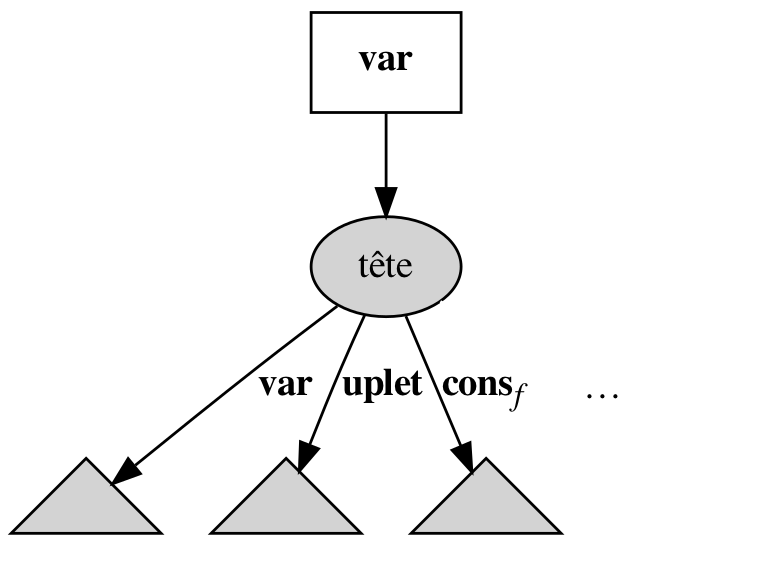
\includegraphics[scale=0.12]{graphs/crit1_1}
	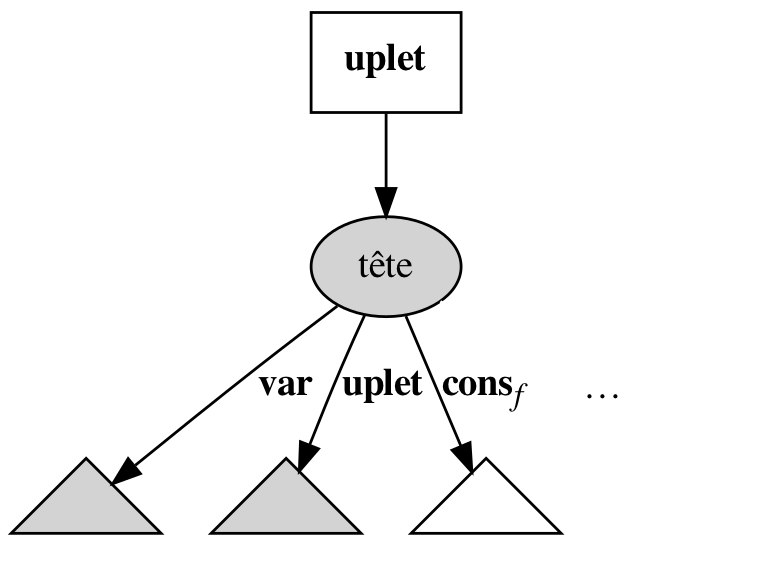
\includegraphics[scale=0.12]{graphs/crit1_2}
	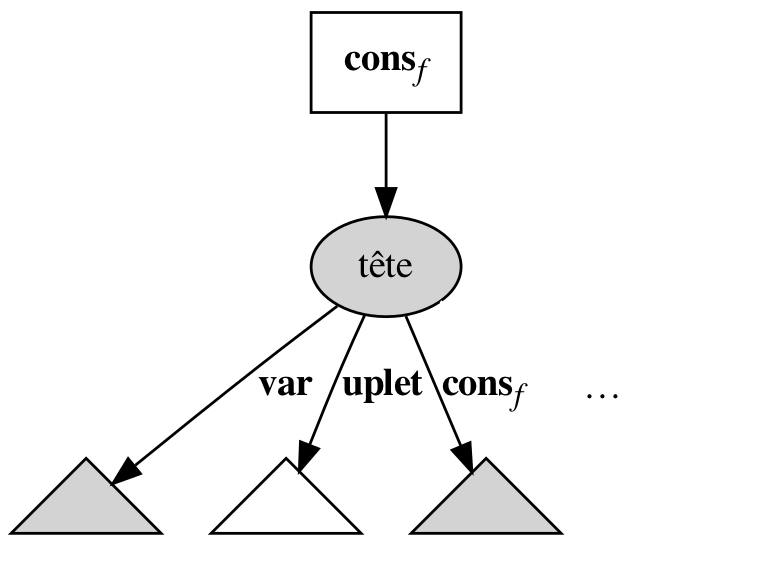
\includegraphics[scale=0.12]{graphs/crit1_3}
\end{figure}
\end{frame}

%============================================================

\begin{frame}{Deuxième critère}
\scriptsize
\begin{align*}
		\mu_g (\nu^\# \rightarrow \nu) &=
		\mu_g' (\nu^\#)
	\\
		\mu_g (\nu) &=
		0
	\\
		\mu_g' (\mset{\nu_1, \dots, \nu_n}) &=
		\sum_{i=1}^n \mu_g'' (\nu_i)
	\\
		\mu_g'' (\nu) &=
		1 &&
		\text{si } [\nu] = g
	\\
		\mu_g'' (\nu) &=
		0 &&
		\text{sinon}
\end{align*}
\medskip
\begin{mathpar}
	\inferrule*
		{[\nu] \notin \{ \bold{var}, \bold{fleche} \}}
		{\nu\ \bold{simple}}
	\and
	\inferrule*
		{\forall i \in \interval 1 n,\ [\nu_i] \neq \bold{var} \\ [\nu] \neq \bold{var}}
		{\mset{\nu_1, \dots, \nu_n} \rightarrow \nu\ \bold{simple}}
\end{mathpar}
\\
\theoreme : Si deux types normalisés bien formés $\nu_1$ et $\nu_2$ sont unifiables et $\nu_1$ simple, on a :
\[ \forall g \neq \bold{var},\ \mu_g (\nu_1) \geqslant \mu_g (\nu_2) \]
\exemples :
\begin{enumerate}
	\item $\mset{int, int} \rightarrow int \nsim_\N \mset{int} \rightarrow float$
	\item $\mset{int} \rightarrow int \nsim_\N \mset{int, int, \alpha} \rightarrow \alpha$
	\item $\mset{int, \mset{} \rightarrow \mset{}} \rightarrow \mset{} \nsim_\N \mset{int, \mset{int} \rightarrow float, int} \rightarrow \alpha$
\end{enumerate}
\end{frame}

%============================================================

\begin{frame}{Deuxième critère — implémentation}
\tiny
\begin{align*}
		\mathrm{encode}^2_g (\nu) &=
		(\mathrm{vars\mathhyphen echine} (\nu), \mu_g (\nu))
	\\
		\mathrm{vars\mathhyphen echine} (\nu) &=
		\bold{F} &&
		\text{si } \mu^3 (\nu) = 0
	\\
		\mathrm{vars\mathhyphen echine} (\nu) &=
		\bold{V} &&
		\text{sinon}
\end{align*}
\begin{align*}
		\mathrm{compat}^2_g ((\bold{V}, \mu_1), (\bold{V}, \mu_2)) &=
		\bold{V}
	\\
		\mathrm{compat}^2_g ((\bold{V}, \mu_1), (\bold{F}, \mu_2)) &=
		\bold{V} &&
		\text{si } \mu_1 \leqslant \mu_2
	\\
		\mathrm{compat}^2_g ((\bold{V}, \mu_1), (\bold{F}, \mu_2)) &=
		\bold{F} &&
		\text{sinon}
	\\
		\mathrm{compat}^2_g ((\bold{F}, \mu_1), (\bold{V}, \mu_2)) &=
		\bold{V} &&
		\text{si } \mu_2 \leqslant \mu_1
	\\
		\mathrm{compat}^2_g ((\bold{F}, \mu_1), (\bold{V}, \mu_2)) &=
		\bold{F} &&
		\text{sinon}
\end{align*}
\begin{figure}[h]
	\centering
	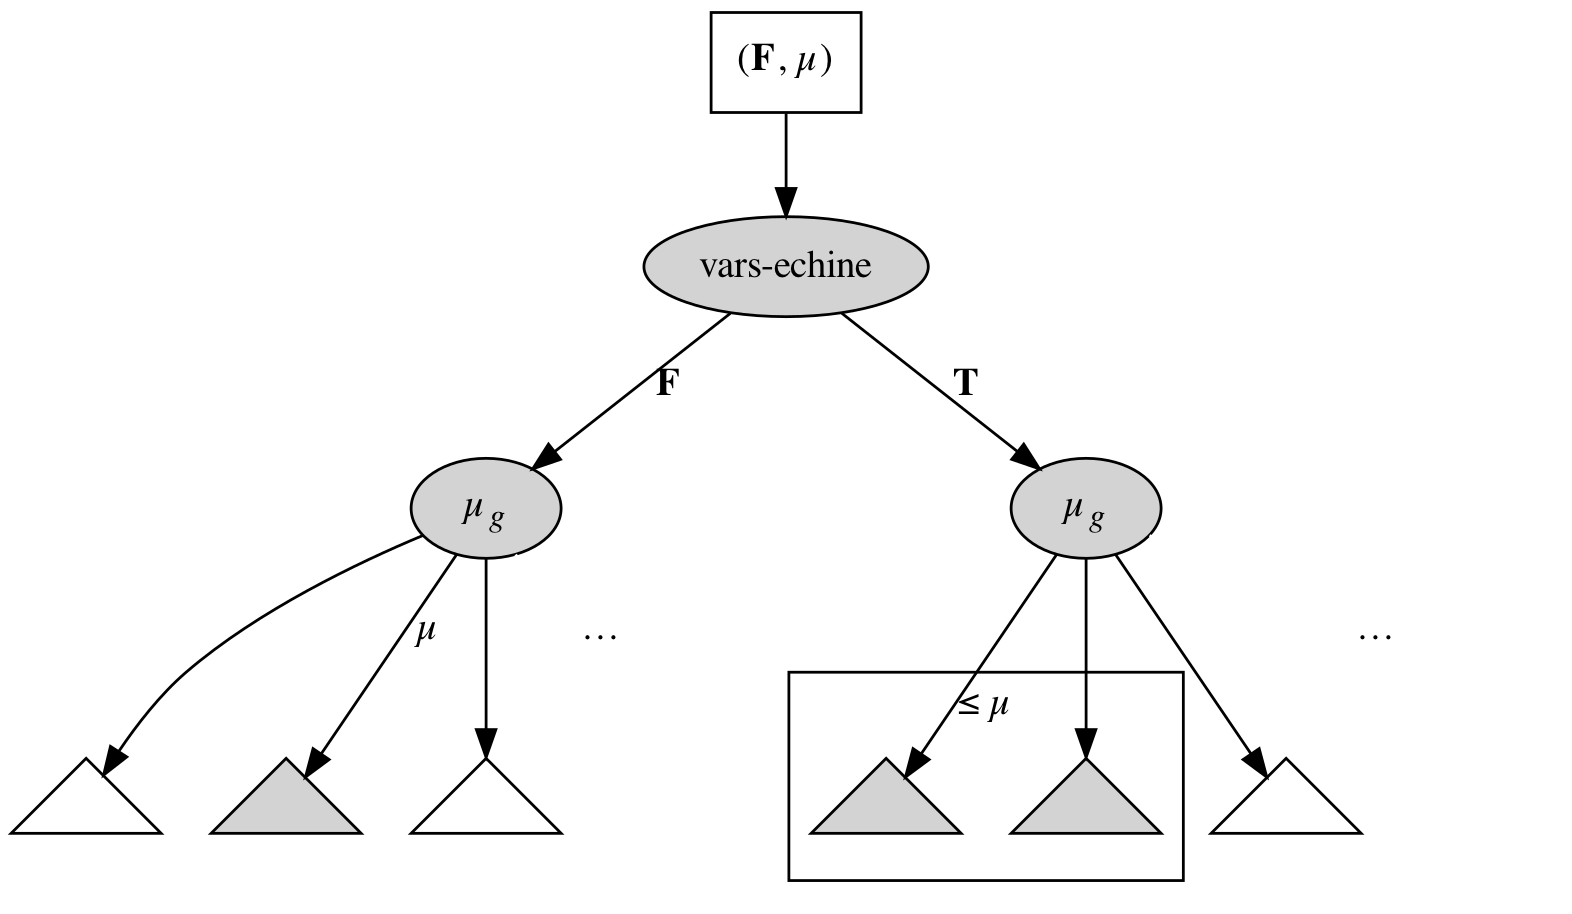
\includegraphics[scale=0.09]{graphs/crit2_1}
	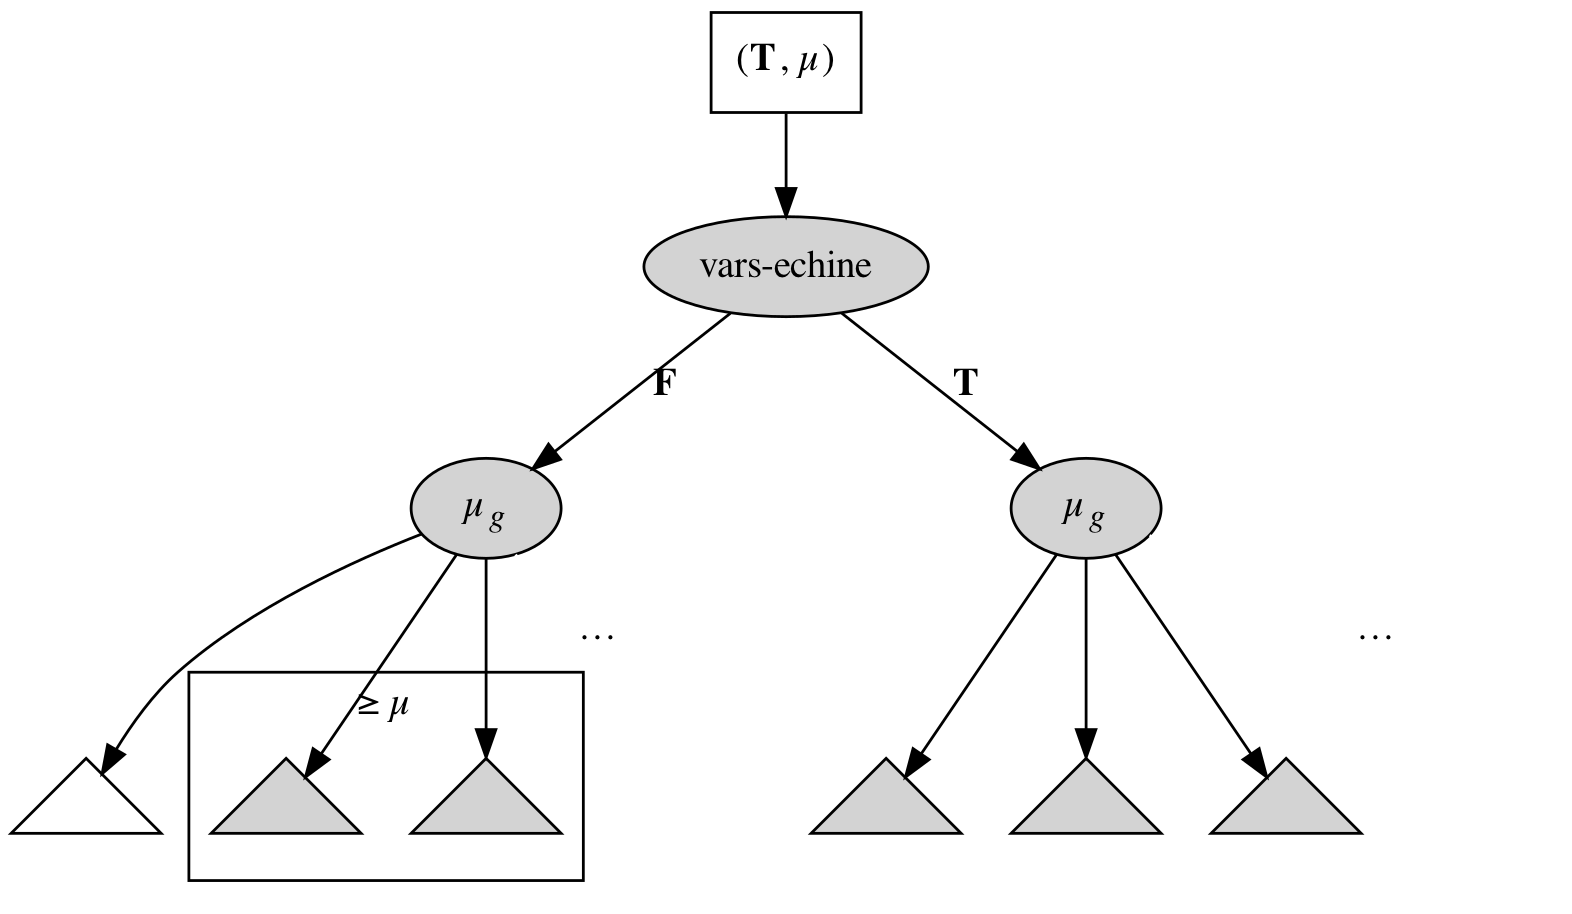
\includegraphics[scale=0.09]{graphs/crit2_2}
\end{figure}
\end{frame}

%============================================================

\begin{frame}{Deuxième critère — en parallèle}
\footnotesize
\[ \mathrm{encode}^2 (\nu) = \left( \mathrm{vars\mathhyphen base} (\nu), \msetG_bigplus_{g \notin \{ \bold{var}, \bold{uplet} \}} \msetG_bigplus_{\interval 1 {\mu_g (\nu)}} \mset{g} \right) \]
\begin{align*}
		\mathrm{compat}^2 ((\bold{V}, {g}^\#_1), (\bold{V}, {g}^\#_2)) &=
		\bold{V}
	\\
		\mathrm{compat}^2 ((\bold{V}, {g}^\#_1), (\bold{F}, {g}^\#_2)) &=
		\bold{V} &&
		\text{si } {g}^\#_1 \subseteq^\#_\G {g}^\#_2
	\\
		\mathrm{compat}^2 ((\bold{V}, {g}^\#_1), (\bold{F}, {g}^\#_2)) &=
		\bold{F} &&
		\text{sinon}
	\\
		\mathrm{compat}^2 ((\bold{F}, {g}^\#_1), (\bold{V}, {g}^\#_2)) &=
		\bold{V} &&
		\text{si } {g}^\#_2 \subseteq^\#_\G {g}^\#_1
	\\
		\mathrm{compat}^2 ((\bold{F}, {g}^\#_1), (\bold{V}, {g}^\#_2)) &=
		\bold{F} &&
		\text{sinon}
\end{align*}
\end{frame}

%============================================================

\begin{frame}{Trie}
\small
\begin{mathpar}
	\inferrule*
		{N \subseteq \N}
		{\bold{feuille} (N) \in \mathscr{T}}
	\and
	\inferrule*
		{crit \in \mathscr{C}_\mathscr{D} \\ fils \in \mathscr{F} (\mathscr{D}, \mathscr{T})}
		{\bold{noeud}_\mathscr{D} (crit, fils) \in \mathscr{T}}
\end{mathpar}
\\~\\
\exemple : $\bold{noeud}_{\mathscr{D}^1} (\mathrm{crit}^1, g \mapsto \bold{noeud}_{\mathscr{D}^2} (\mathrm{crit}^2, (b, g^\#) \mapsto \bold{feuille} (\{ \})))$
\end{frame}

%============================================================

\begin{frame}{Trie — ajout et recherche}
\scriptsize
\begin{align*}
		\mathrm{trie\mathhyphen ajoute} (\bold{feuille} (N), \nu) &=
		\bold{feuille} (N \cup \{ \nu \})
	\\
		\mathrm{trie\mathhyphen ajoute} (\bold{noeud}_\mathscr{D} (crit, fils), \nu) &=
		\bold{noeud}_\mathscr{D} (crit, d \mapsto \mathrm{trie\mathhyphen ajoute}_\mathscr{D}' (crit, fils, \nu, d))
\end{align*}
\begin{align*}
		\mathrm{trie\mathhyphen ajoute}_\mathscr{D}' ((encode, \_), fils, \nu, d) &=
		\mathrm{trie\mathhyphen ajoute} (fils (d), \nu) &&
		\text{si } d = encode (\nu)
	\\
		\mathrm{trie\mathhyphen ajoute}_\mathscr{D}' ((encode, \_), fils, \nu, d) &=
		fils (d) &&
		\text{sinon}
\end{align*}
\begin{align*}
		\mathrm{trie\mathhyphen cherche} (\bold{feuille} (N), \nu) &=
		N
	\\
		\mathrm{trie\mathhyphen cherche} (\bold{noeud}_\mathscr{D} ((encode, compat), fils), \nu) &=
		\bigcup_{\mathclap{{d \in \mathscr{D} \mid compat (d, encode (\nu)) = \bold{T}}}} \mathrm{trie\mathhyphen cherche} (fils (d), \nu)
\end{align*}
\end{frame}

%============================================================

\begin{frame}[fragile=singleslide]\frametitle{Trie — Interface OCaml}
\footnotesize
\begin{minted}{ocaml}
module type FEATURE = sig
  type t
  val compute : Type.t -> t
  val compare : t -> t -> Int.t
  val compatible : query:t -> data:t -> Bool.t
end

module type NODE = sig
  type t
  val empty : t
  val add : Type.t -> t -> t
  val iter_with : Type.t -> t -> Type.t Iter.t
end

module Leaf : NODE
module Node (Feat : FEATURE) (Sub : NODE) : NODE
\end{minted}
\end{frame}

%============================================================

\end{document}